\documentclass[10pt, unicode]{beamer}
\usepackage{fontspec}
\usepackage{polyglossia}
\setdefaultlanguage{english}
\usepackage{amsmath}
\usepackage{amssymb}
\usepackage{mathtools}
\usepackage{lmodern}
\usepackage{graphics}
\usepackage{graphicx}
\usepackage{subcaption}
\usepackage{relsize}

\usepackage{algorithm}
\usepackage{algpseudocode}
\newenvironment{algo}[1][]
  {\begin{algorithm}[#1]
     \selectlanguage{english}
     \floatname{algorithm}{Алгоритм}
  }
  {\end{algorithm}}
\graphicspath{{images/}}

\usepackage{float}
\usepackage{caption}
\usepackage{newfloat}

\DeclareMathOperator{\sech}{sech}
\setsansfont{Fira Sans}
\title{Генерация текстурного меша и упаковка полигональных текстур в атлас}
\author[Терехов Д.Е.]{Студент группы Б8403а Терехов Дмитрий Евгеньевич\\
Руководитель:\\
Старший преподаватель\\
Александр Сергеевич Кленин}
%\date{20 июня 2019}
\date{}
\usetheme[progressbar=frametitle, numbering=fraction]{metropolis}
\makeatletter
        \setlength{\metropolis@progressinheadfoot@linewidth}{2pt}
    \makeatother
\date{\today}
\begin{document}
    \begin{frame}
        \titlepage
        \thispagestyle{empty}
    \end{frame}
    \begin{frame}
        \frametitle{Студия "Game Forest"}
        \begin{figure}[H]
            \centering
            \begin{subfigure}[l]{0.50\linewidth}
                \centering
                
\includegraphics[scale=0.15]{GAMEFOREST.png}
            \end{subfigure}
            \begin{subfigure}{0.49\linewidth}
                \begin{subfigure}{\linewidth}
                    \centering
                    
\includegraphics[scale=0.15]{TSD4.jpg}
                \end{subfigure}
                \begin{subfigure}{\linewidth}
                    \centering
                    
\includegraphics[scale=0.260]{GD.jpg}
                \end{subfigure}
            \end{subfigure}
        \end{figure}
    \end{frame}
    \begin{frame}
        \frametitle{Игровой движок Citrus}
        \begin{figure}
            \centering
            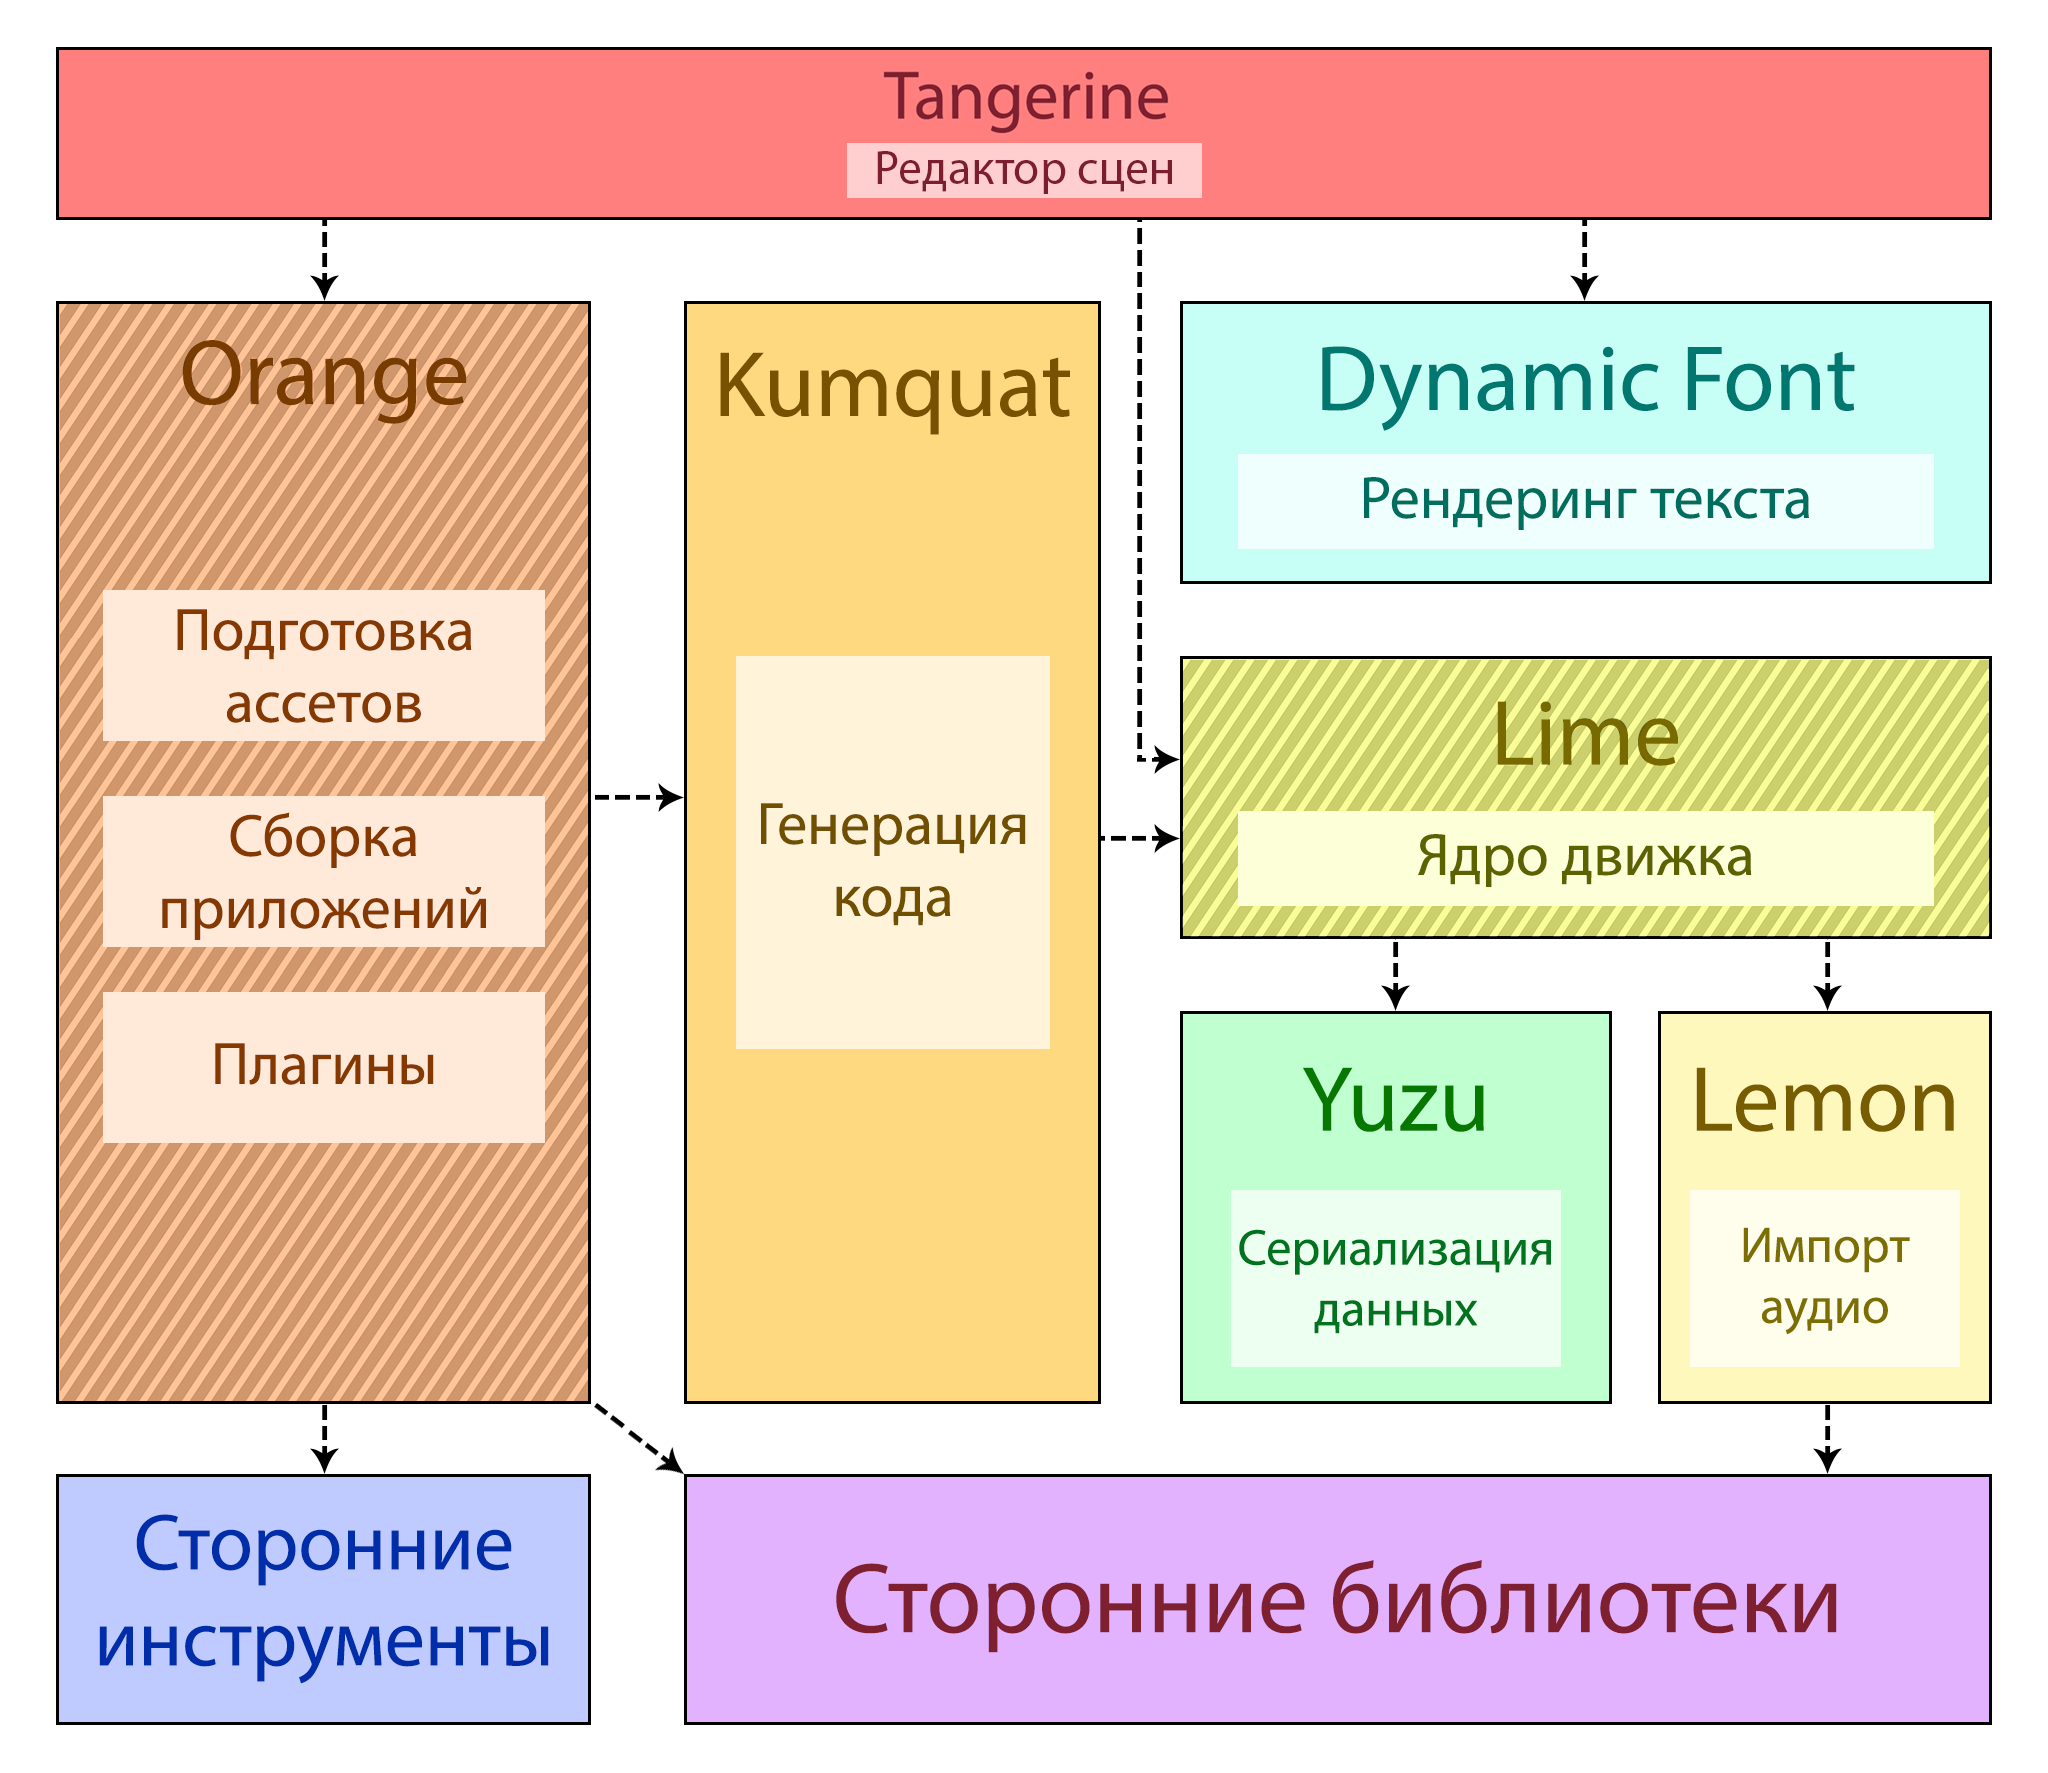
\includegraphics[width=\linewidth, height=.9\textheight, keepaspectratio]{CtrusArchitecture2.png}
        \end{figure}
    \end{frame}
    \begin{frame}
        \frametitle{Упаковка текстур в атлас}
        \begin{itemize}
            \item Жадный алгоритм
            \item Генерация текстурного меша, полигональная упаковка
        \end{itemize}
        \begin{figure}
            \centering
            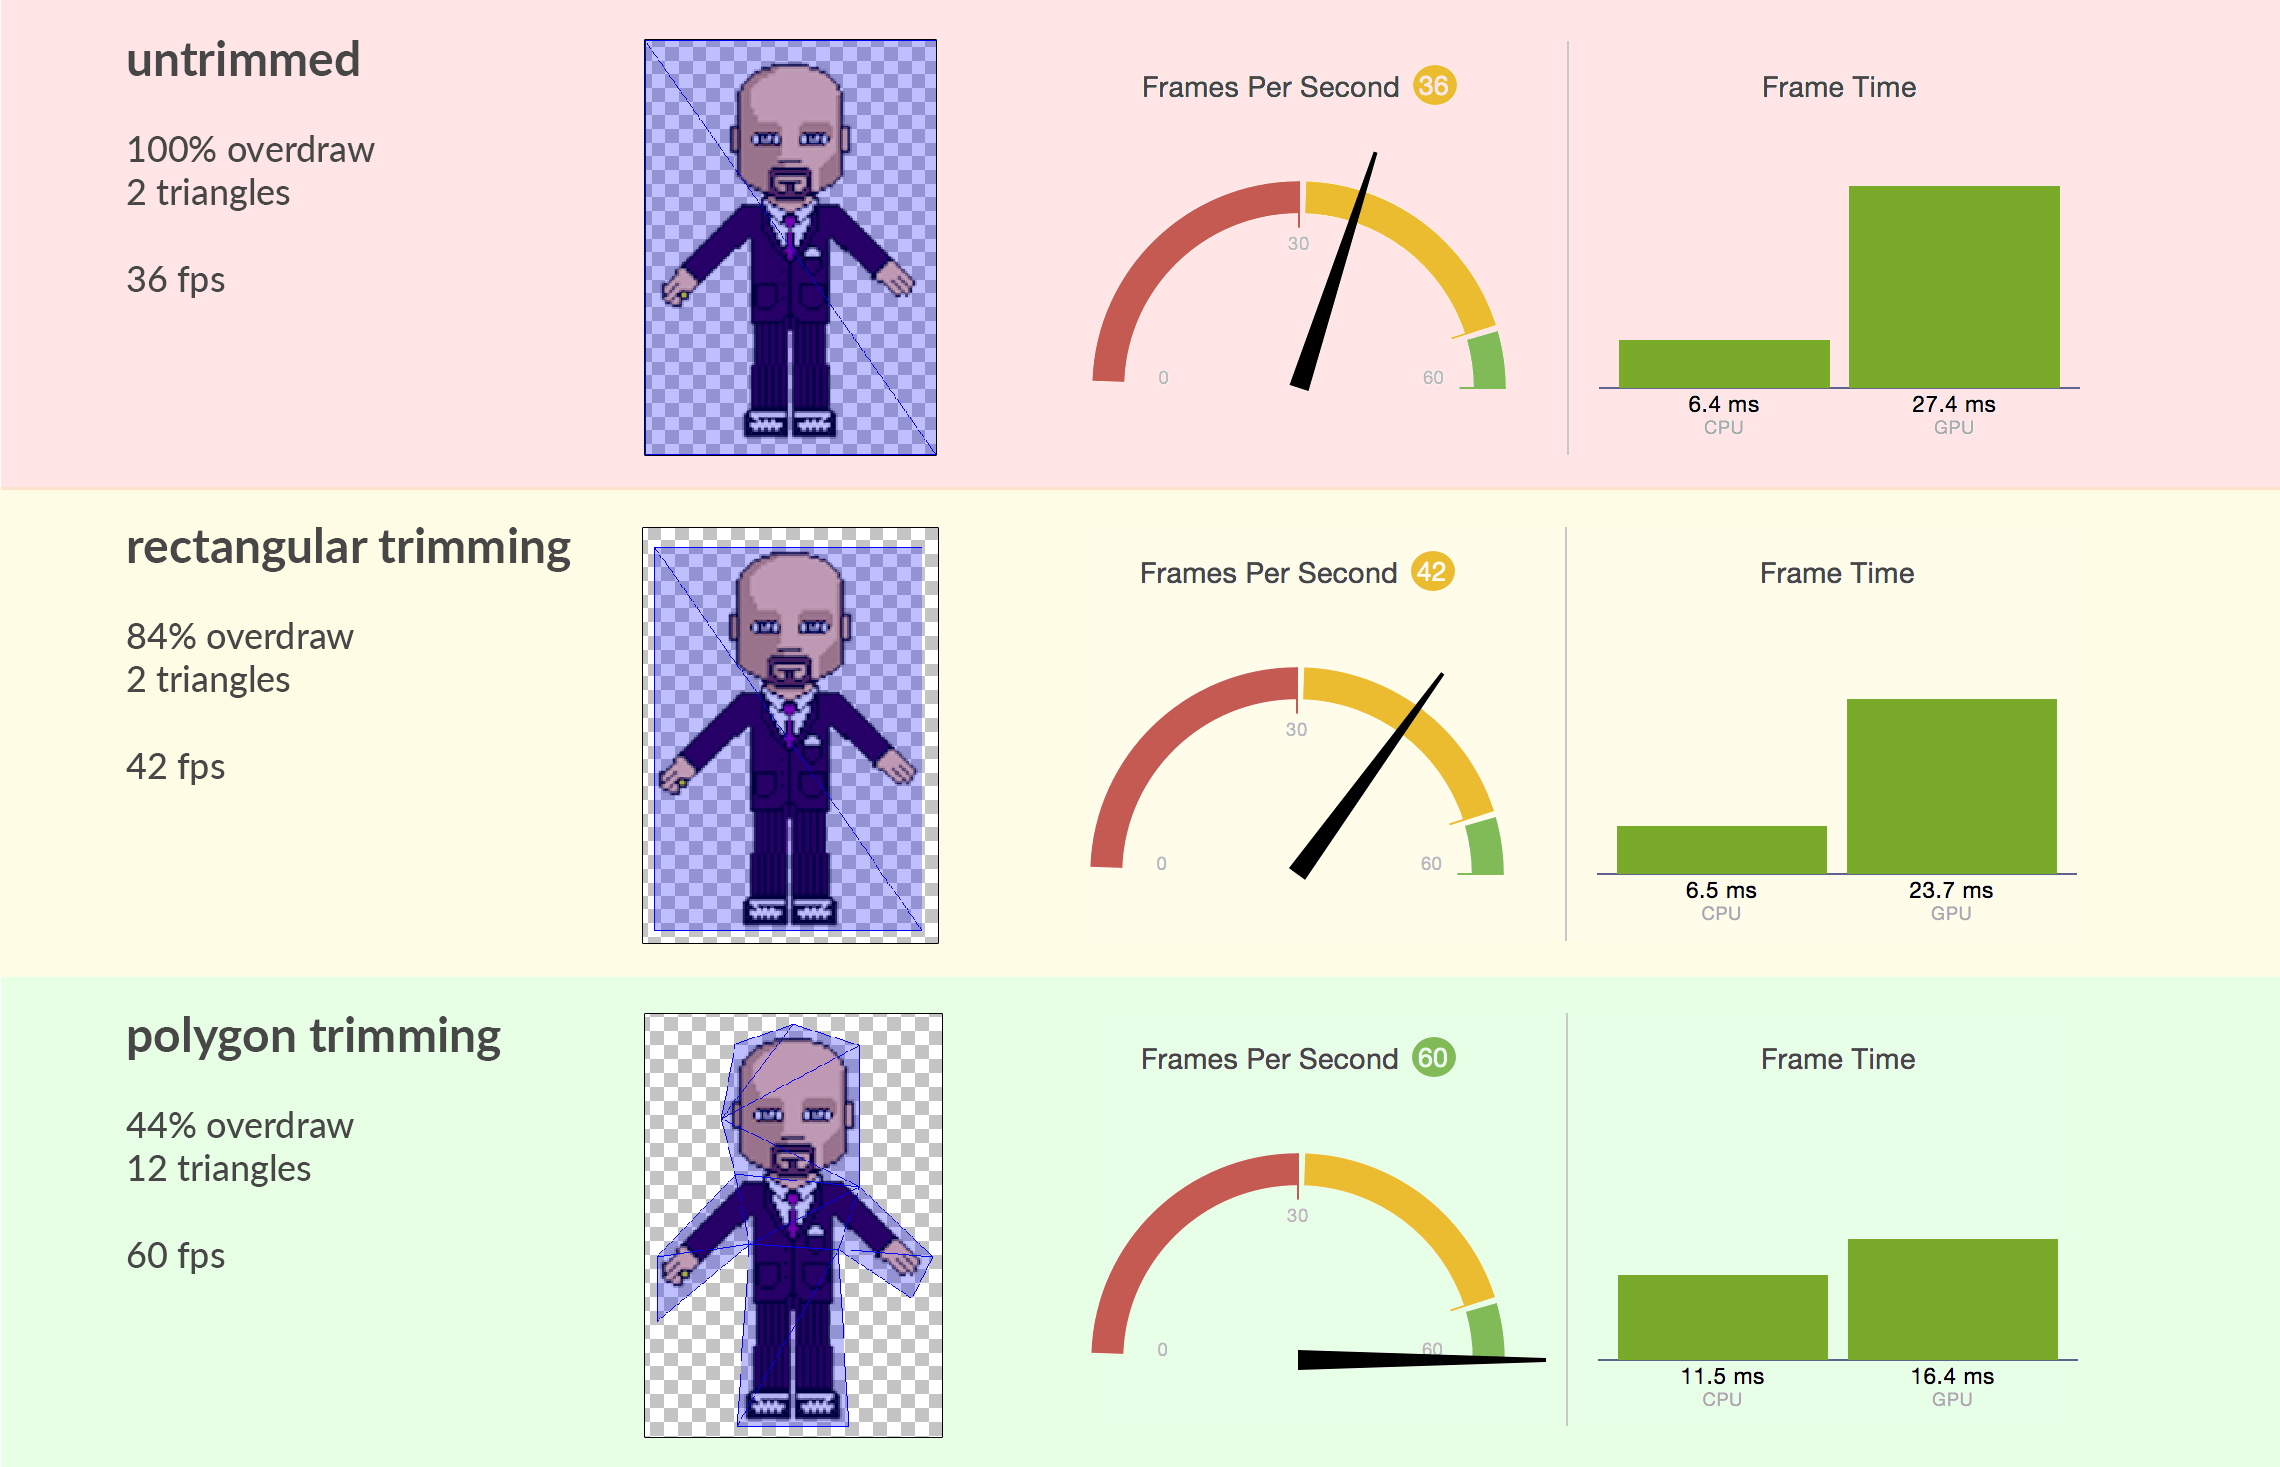
\includegraphics[width=\linewidth, keepaspectratio]{SuperPacking.png}
        \end{figure}
    \end{frame}
    \begin{frame}
        \frametitle{DistortionMesh}
        \begin{itemize}
            \item Структура меша -- регулярная сетка
        \end{itemize}
        \begin{figure}
            \centering
            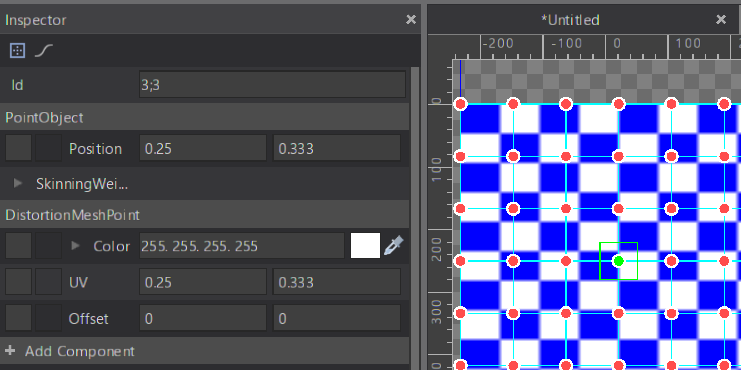
\includegraphics[scale=0.5]{DistortionMesh.png}
        \end{figure}
    \end{frame}
    \begin{frame}
        \frametitle{Цели}
        Цели:
        \begin{itemize}
            \item Оптимизировать упаковку текстур в атлас
            \item Позволить динамически задавать структуру меша
        \end{itemize}
    \end{frame}
    \begin{frame}
        \frametitle{Этапы полигональной упаковки в атлас}
        \begin{itemize}
            \item Трассировка контура
            \item Генерация невыпуклой оболочки -- аппроксимация контура полигоном
            \item Генерация меша из невыпуклой оболочки
            \item Упаковка в атлас
        \end{itemize}
    \end{frame}
    \begin{frame}
        \frametitle{Трассировка контура}
        Алгоритмы трассировки контура начинают с какого-то стартового пикселя и пиксель за пикселем обходят границу 
        объекта на текстуре. Алгоритмы отличаются способом перехода к следующему граничному пикселю. 
        \begin{itemize}
            \item Square Tracing -- имеет направление. Осуществляются повороты и шаг вперед
            \item Moor-neighborhood Tracing. Обходит окрестность пикселя (8 соседних пикселей)
        \end{itemize}
    \end{frame}
    \begin{frame}[fragile]
        \frametitle{Генерация невыпуклой оболочки}
        \begin{itemize}
            \item Аппроксимация контура полигоном
            \item Алгоритм Висвалингэма
        \end{itemize}
        \begin{center}
            \scalebox{0.85}{
                \begin{minipage}{\linewidth}
                    \begin{algo}[H]
                        \caption{Visvalingam polyline simplification}
                        \begin{algorithmic}[1]
                            \Procedure{Visvalingam}{$B, maxArea$}
                                \State $heap \gets MinHeap(B)$
                                \While{$heap \not= \emptyset$}
                                    \State $min \gets \min\left(heap\right)$
                                    \State $heap \gets heap \setminus \{min\}$
                                    \If{$Area(min) \leq maxArea$}
                                        \State $B \gets B \setminus \{min\}$
                                        \State $Update(heap, Next(min))$
                                        \State $Update(heap, Prev(min))$
                                    \EndIf
                                \EndWhile
                                \State \textbf{return} $B$
                            \EndProcedure
                        \end{algorithmic}
                    \end{algo}
                \end{minipage}
            }
        \end{center}
    \end{frame}
    \begin{frame}
        \frametitle{Триангуляция Делоне}
        \begin{itemize}
            \item Невырожденная Триангуляция Делоне единственна
            \item Алгоритмы уточнения триангуляции Делоне для улучшения качества треугольников
            \item Триангуляция Делоне с ограничениями для вставки структурных отрезков
        \end{itemize}
        \begin{figure}
            \centering
            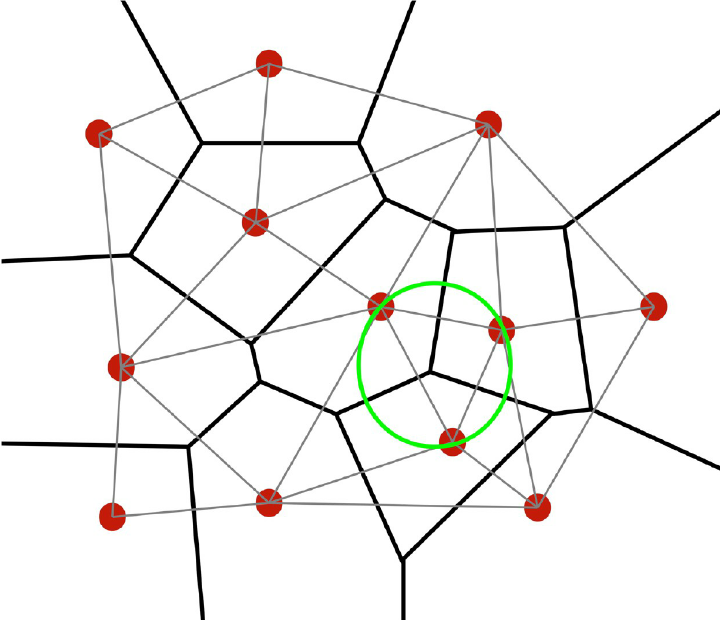
\includegraphics[scale=0.25]{DelaunayAndVoronoi.png}
        \end{figure}
    \end{frame}
    \begin{frame}
        \frametitle{Флип}
        \begin{figure}[H]
            \centering
            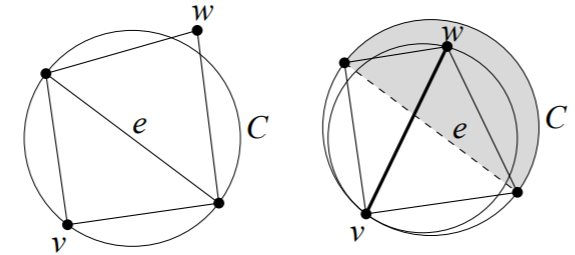
\includegraphics[width=\linewidth, keepaspectratio]{FlipLemma.jpg}
        \end{figure}
    \end{frame}
    \begin{frame}
        \frametitle{Локализация вершины}
        \begin{figure}[H]
            \centering
            \begin{subfigure}{0.49\linewidth}
                \centering
                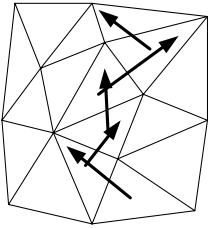
\includegraphics[scale=0.5]{SeparatingEdge.png}
                \caption{Переход через разделяющее ребро}
            \end{subfigure}
            \begin{subfigure}{0.49\linewidth}
                \centering
                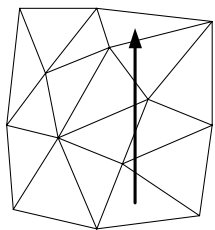
\includegraphics[scale=0.5]{ThrougSegmentIntersection.jpg}
                \caption{Переход вдоль сегмента}
            \end{subfigure}
        \end{figure}
    \end{frame}
    \begin{frame}
        \frametitle{Добавление вершины, лежащей внутри триангуляции}
        Алгоритм Бойера-Ватсона
        \begin{figure}[H]
            \centering
            \begin{subfigure}{0.49\linewidth}
                \centering
                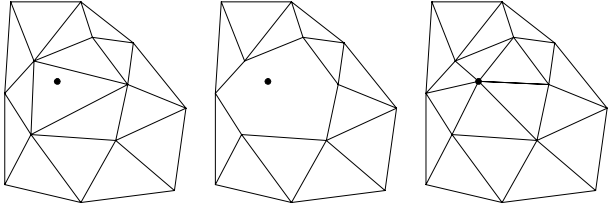
\includegraphics[scale=0.4, angle=-90]{BowyerWatson.png}
            \end{subfigure}
            \begin{subfigure}[l]{0.49\linewidth}
                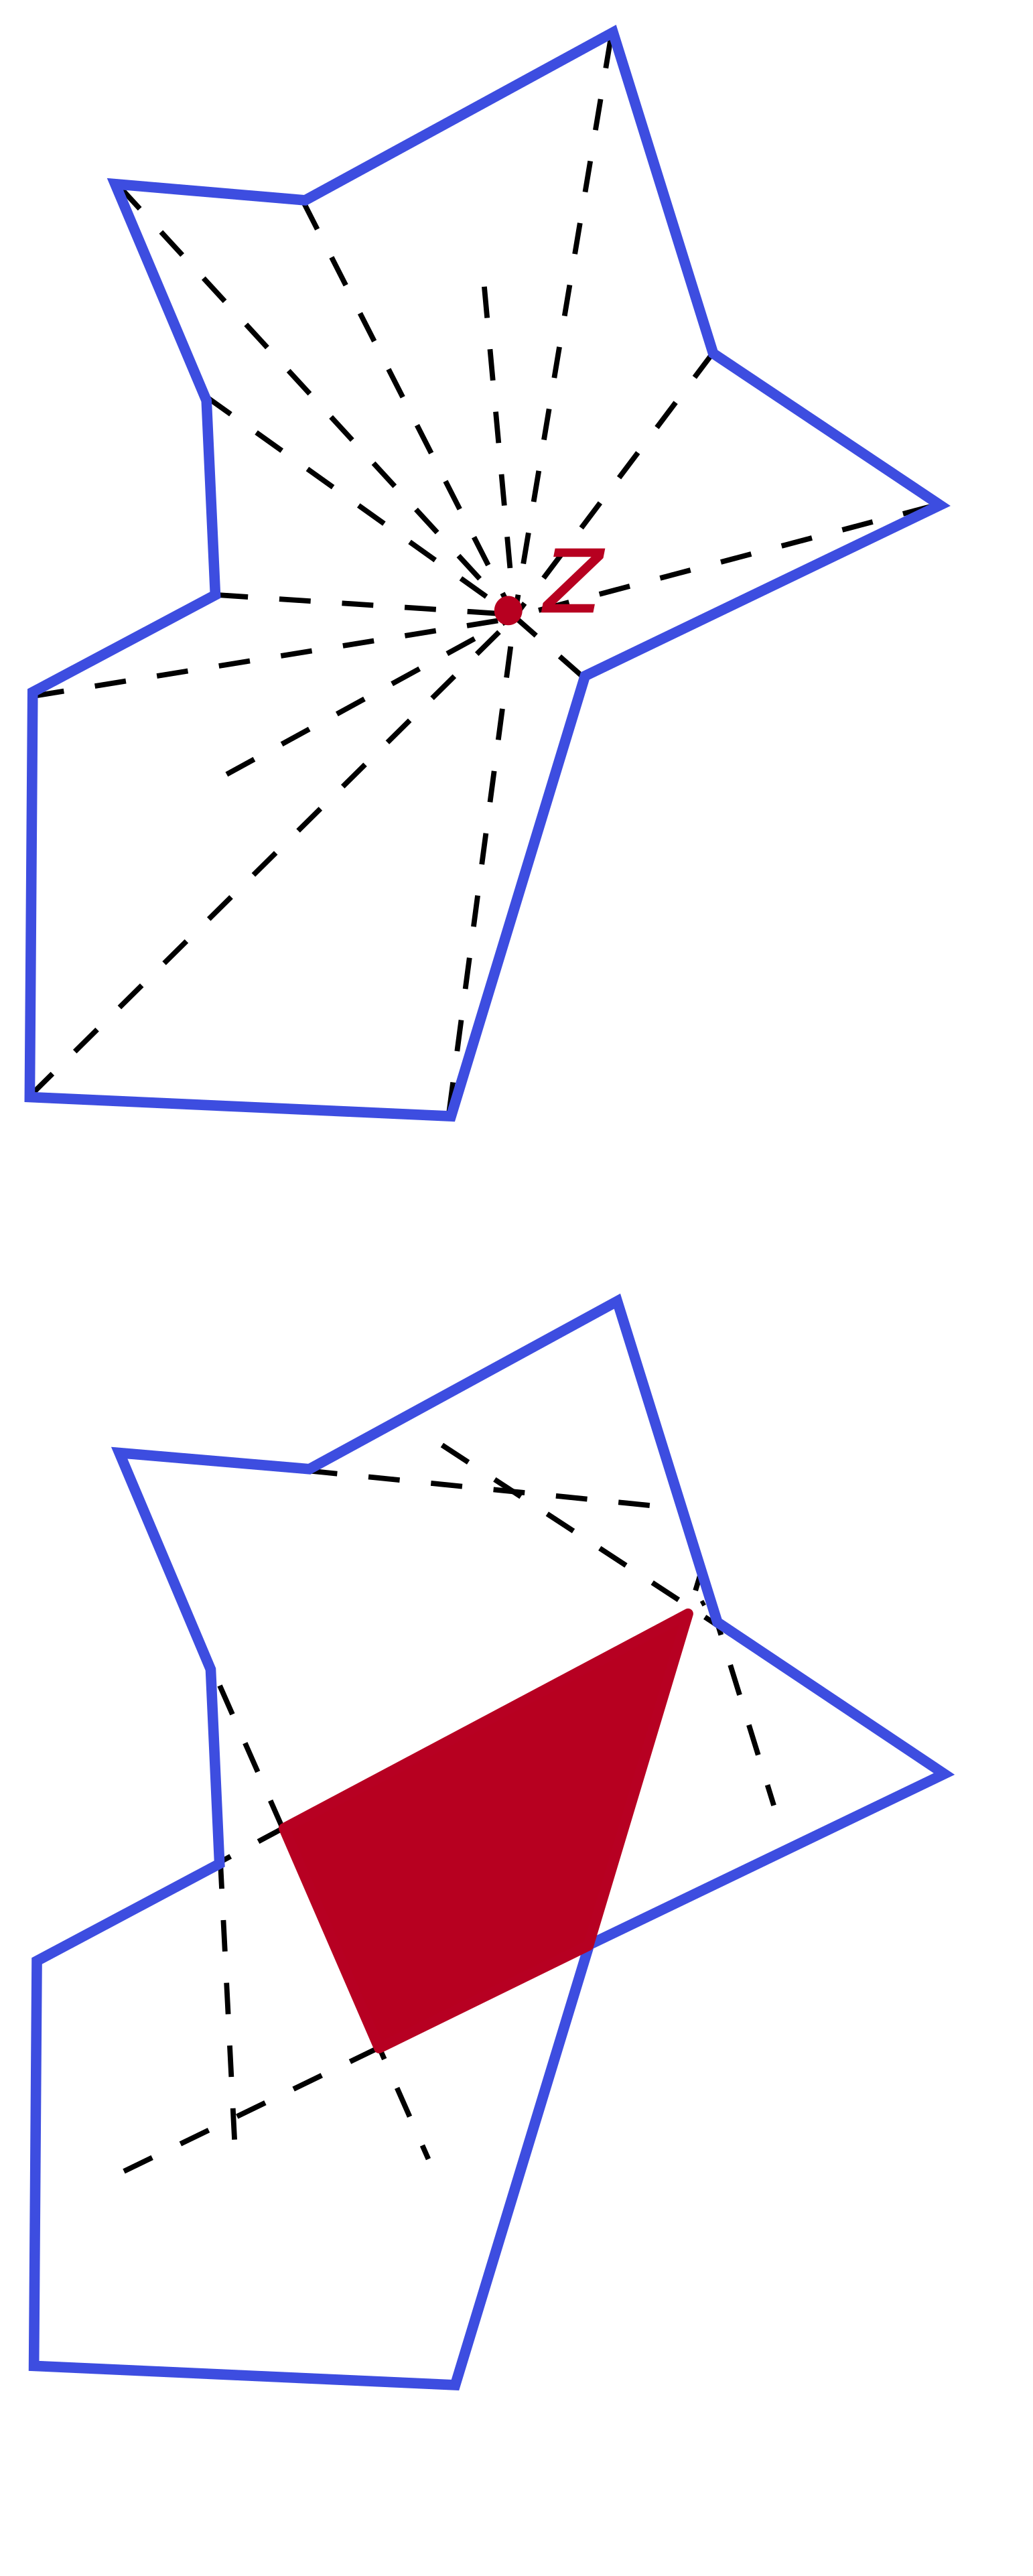
\includegraphics[scale=0.225]{StarShapedPolygon.png}
            \end{subfigure}
        \end{figure}
    \end{frame}
    \begin{frame}
        \frametitle{Добавление вершины, лежащей снаружи триангуляции}
        Достраивание до выпуклой оболочки с дальнейшей проверкой на условие Делоне и выполнением необходимых перестроений
        \begin{figure}[H]
            \centering
            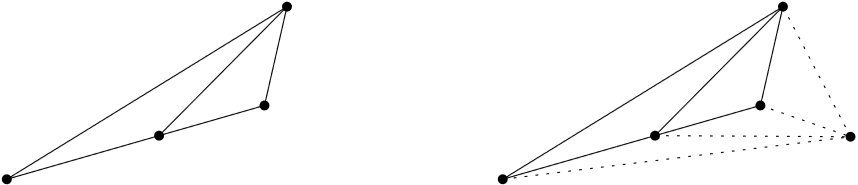
\includegraphics[scale=0.5]{AddOutOfTriangulationVertex.png}
        \end{figure}
    \end{frame}
    \begin{frame}
        \frametitle{Удаление вершины, лежащей внутри триангуляции}
        \begin{itemize}
            \item Образуется полигональная дыра. Ear Clipping $O(n^2)$, Seidel $O(n\log n)$ или $O(n\log n)$, 
            Chazelle $O(n)$*
            \item Проверка на условие Делоне, выполнение необходимых перестроений
        \end{itemize}
        \begin{figure}[H]
            \centering
            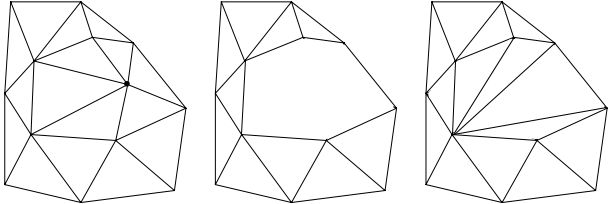
\includegraphics[scale=0.5]{DeleteInsideVertex.png}
        \end{figure}
    \end{frame}
    \begin{frame}
        \frametitle{Удаление граничной вершины}
        \begin{figure}[H]
            \centering
            \begin{subfigure}{0.33\linewidth}
                \centering
                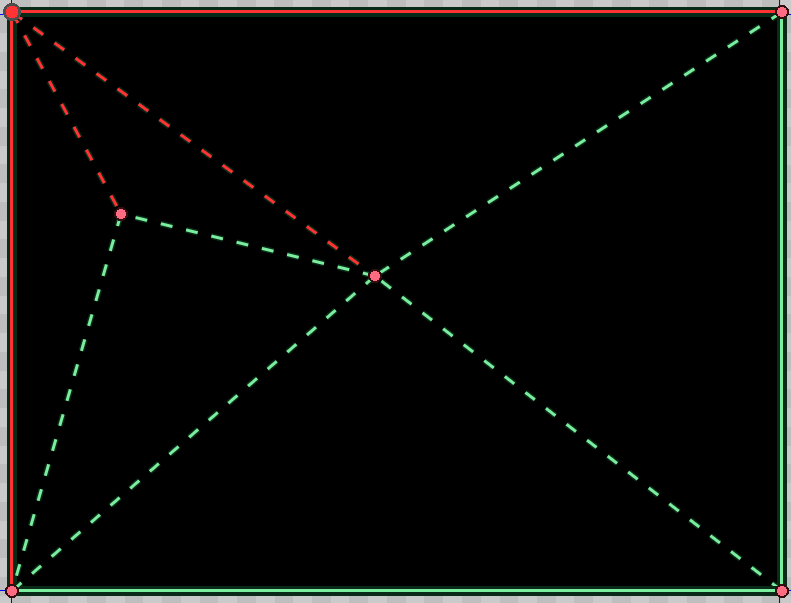
\includegraphics[scale=0.225]{DeleteBoundary1.png}
            \end{subfigure}
            \begin{subfigure}[H]{0.33\linewidth}
                \centering
                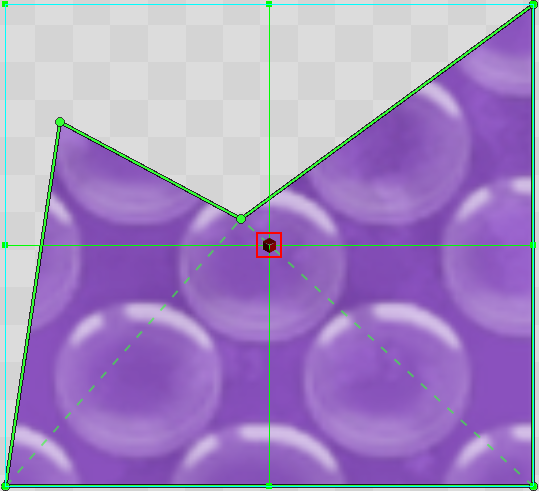
\includegraphics[scale=0.225]{DeleteBoundary2.png}
            \end{subfigure}
            \begin{subfigure}{0.33\linewidth}
                \centering
                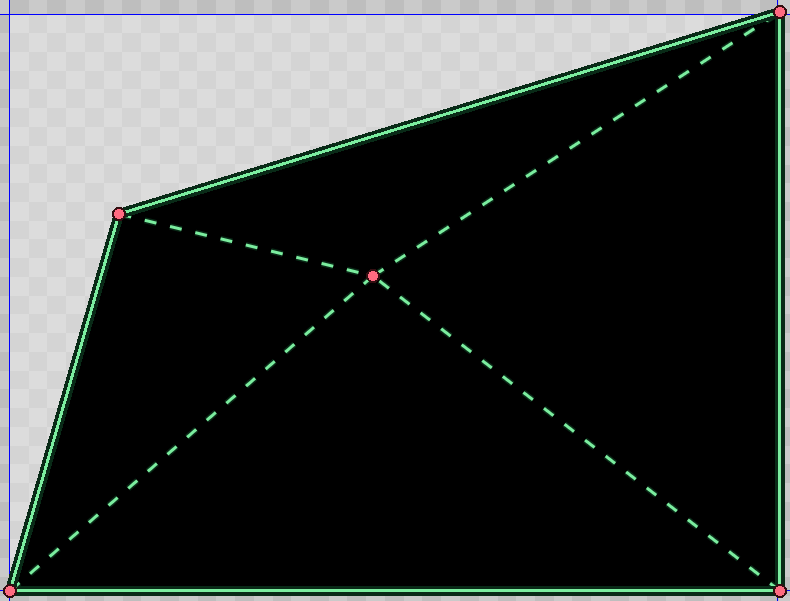
\includegraphics[scale=0.225]{DeleteBoundary3.png}
            \end{subfigure}
        \end{figure}
    \end{frame}
    \begin{frame}
        \frametitle{Триангуляция Делоне с ограничениями}
        \begin{figure}[H]
            \centering
            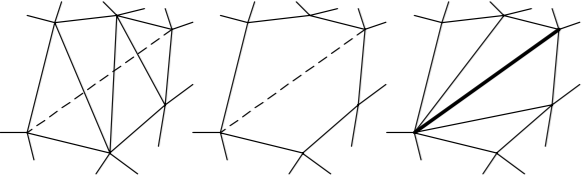
\includegraphics[width=\linewidth, keepaspectratio]{DestroyAndBuild.png}
        \end{figure}
    \end{frame}
    \begin{frame}
        \frametitle{PolygonMesh}
        \begin{figure}[H]
            \centering
            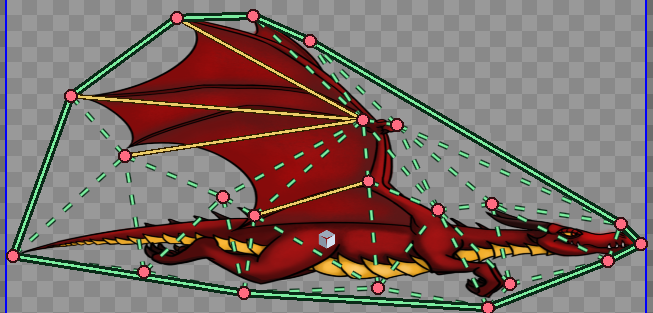
\includegraphics[scale=0.8]{PGMW.png}
        \end{figure}
    \end{frame}
    \begin{frame}
        \frametitle{Жадная упаковка. Алгоритм гильотины}
        \begin{itemize}
            \item Эвристика выбора свободного прямоугольника
            \item Эвристика выбора разреза
        \end{itemize}
        \begin{figure}[H]
            \centering
            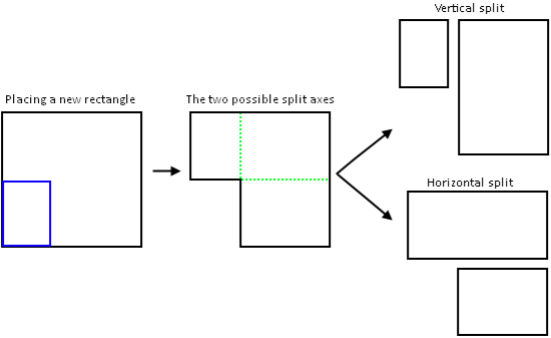
\includegraphics[width=\linewidth, keepaspectratio]{Guillotine.png}
        \end{figure}
    \end{frame}
    \begin{frame}
        \frametitle{Полигональная упаковка. Генетический алгоритм}
        Генотип -- количество контейнеров + пары (позиция, поворот), описывающие меши
        \[
            f_cost = \alpha \cdot intersectionArea  + \beta \cdot outsideArea
        \]
    \end{frame}
    \begin{frame}
        \frametitle{Реализация}
        Объем написанного кода 3,302 ++  959 -- (30 коммитов) в тестовом репозитории, 1200 ++, 100-- (15 коммитов) 
        в репозитории Citrus. Реализованы методы работы со структурой меша (триангуляцией множества точек) для 
        виджета PolygonMesh, методы генерации текстурного меша, генетический алгоритм и алгоритм гильотины для упаковки текстур в атласы.  
    \end{frame}
    \begin{frame}
        \frametitle{Заключение}
        По результатам работы было проведено тестирование, ревью кода и перенос кода в рабочую копию игрового движка 
        Citrus
    \end{frame}
\end{document}\frametitle{Триангуляция Делоне}
